\documentclass[tikz,border=4pt]{standalone}
% Paleta y fuentes compartidas por el libro y las figuras (única fuente de verdad).
\RequirePackage{xcolor}
\definecolor{oxido}{HTML}{B7410E}
\definecolor{cobre}{HTML}{D27D2D}
\definecolor{carbon}{HTML}{2B2B2B}
\definecolor{azul}{HTML}{1F5F8B}
\definecolor{arena}{HTML}{F4EDE4}

\usepackage{fontspec}
\setsansfont{FiraSans}[Extension=.otf,UprightFont=*-Regular,BoldFont=*-Bold,ItalicFont=*-Italic,BoldItalicFont=*-BoldItalic]
\setmonofont{FiraMono}[Extension=.otf,UprightFont=*-Regular,BoldFont=*-Medium]
\usetikzlibrary{positioning,arrows.meta,calc,fit}
\begin{document}
\sffamily\small
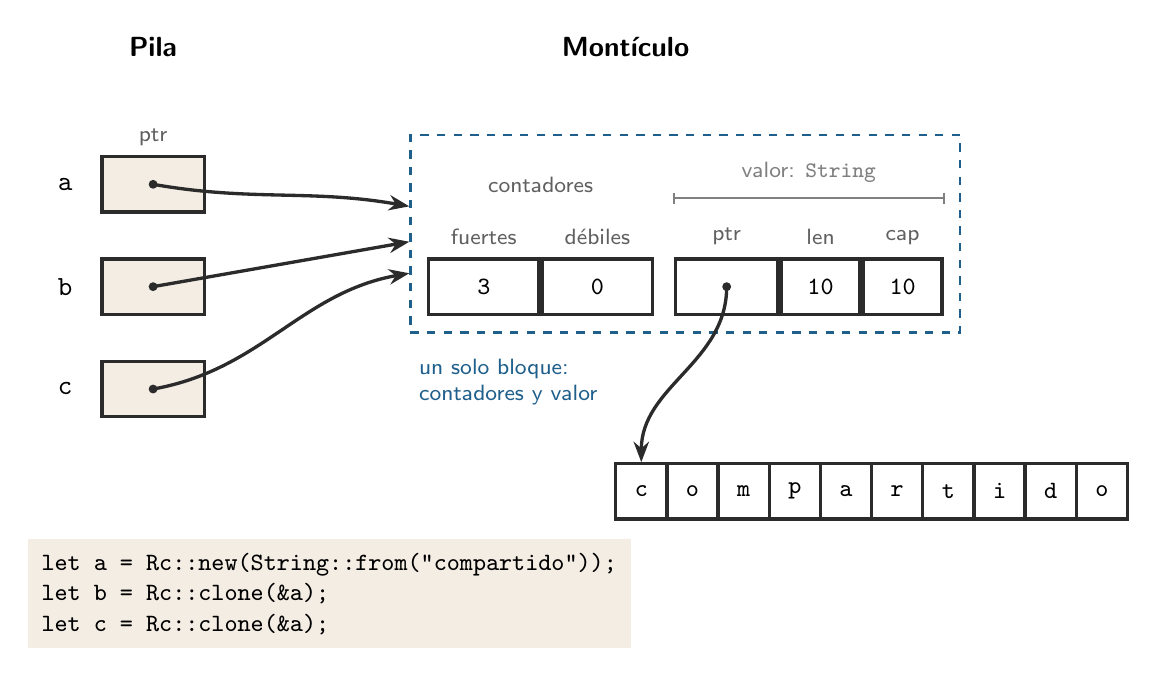
\begin{tikzpicture}[
  celda/.style={draw=carbon,minimum height=7mm,minimum width=13mm,font=\ttfamily\small},
  rotulo/.style={font=\sffamily\footnotesize\color{carbon!75}},
  >={Stealth[length=2.6mm]}]
  % Pila: tres Rc
  \node[font=\sffamily\bfseries] at (0,1.75) {Pila};
  \foreach \n [count=\i from 0] in {a,b,c} {
    \node[celda,fill=arena,very thick] (p\i) at (0,-\i*1.3) {};
    \node[anchor=east,font=\ttfamily\bfseries] at (-0.9,-\i*1.3) {\n};
  }
  \node[rotulo] at (0,0.6) {ptr};
  % Bloque del Rc en el montículo
  \node[font=\sffamily\bfseries] at (6.0,1.75) {Montículo};
  \node[celda,fill=white,very thick,minimum width=14mm] (f) at (4.2,-1.3) {3};
  \node[celda,fill=white,very thick,minimum width=14mm,anchor=west] (d) at (f.east) {0};
  \node[celda,fill=white,very thick,minimum width=13mm,anchor=west] (vp) at ($(d.east)+(0.25,0)$) {};
  \node[celda,fill=white,very thick,minimum width=10mm,anchor=west] (vl) at (vp.east) {10};
  \node[celda,fill=white,very thick,minimum width=10mm,anchor=west] (vc) at (vl.east) {10};
  \node[rotulo,above=1pt of f] (rf) {fuertes};
  \node[rotulo,above=1pt of d] {débiles};
  \node[rotulo,above=1pt of vp] {ptr};
  \node[rotulo,above=1pt of vl] {len};
  \node[rotulo,above=1pt of vc] (rc) {cap};
  \draw[thick,carbon!60] ($(vp.north west)+(0,0.75)$) -- ($(vc.north east)+(0,0.75)$)
    node[midway,above=2pt,font=\sffamily\footnotesize\color{carbon!80}] (tv) {valor: \texttt{String}};
  \draw[thick,carbon!60] ($(vp.north west)+(0,0.68)$) -- ($(vp.north west)+(0,0.82)$);
  \draw[thick,carbon!60] ($(vc.north east)+(0,0.68)$) -- ($(vc.north east)+(0,0.82)$);
  \node[rotulo,anchor=south] at ($(d.west)+(0,1.07)$) {contadores};
  \node[draw=azul,thick,dashed,inner sep=6pt,fit=(f)(vc)(tv)] (bloque) {};
  % Flechas desde la pila
  \foreach \i in {0,1,2} {
    \fill[carbon] (p\i.center) circle (1.6pt);
  }
  \draw[->,very thick,carbon] (p0.center) to[out=-10,in=170] ($(bloque.west)+(0,0.35)$);
  \draw[->,very thick,carbon] (p1.center) -- ($(bloque.west)+(0,-0.1)$) ;
  \draw[->,very thick,carbon] (p2.center) to[out=10,in=-170] ($(bloque.west)+(0,-0.5)$);
  % Texto del String
  \foreach \l [count=\i from 0] in {c,o,m,p,a,r,t,i,d,o} {
    \node[celda,minimum width=6.5mm,fill=white,very thick] (h\i) at (6.2+\i*0.65,-3.9) {\l};
  }
  \fill[carbon] (vp.center) circle (1.6pt);
  \draw[->,very thick,carbon] (vp.center) to[out=-90,in=90] (h0.north);
  \node[anchor=north west,font=\sffamily\footnotesize,align=left,text=azul] at ($(bloque.south west)+(0,-0.2)$)
    {un solo bloque:\\contadores y valor};
  % Código
  \node[anchor=west,font=\ttfamily\small,align=left,fill=arena,inner sep=5pt]
    at (-1.6,-5.2) {let a = Rc::new(String::from("compartido"));\\let b = Rc::clone(\&a);\\let c = Rc::clone(\&a);};
\end{tikzpicture}
\end{document}
